\documentclass[10pt,a4paper]{article}

\usepackage{natbib}
\usepackage{graphicx}
\usepackage{color}
\usepackage{amsmath} 
\usepackage{amssymb} 
\usepackage{bm} 
\usepackage{hyperref}
\usepackage{tikz}
\usepackage{setspace}

\voffset -0.5in
\oddsidemargin 0.2in
\textheight 24cm
\textwidth 6in
\linespread{1.5}

\newcommand\xqed[1]{%
  \leavevmode\unskip\penalty9999 \hbox{}\nobreak\hfill
  \quad\hbox{#1}}
\newcommand\demo{\xqed{$\triangle$}}

\newcommand{\red}{\textcolor{red}}
\newcommand{\blue}{\textcolor{blue}}

\newcommand{\expect} {{\mathbb{E}}}
\newcommand{\pt} {\tilde{p}}
\newcommand{\nei} {\textrm{ne}}
\newcommand{\alphat} {\tilde{\alpha}}
\newcommand{\betat} {\tilde{\beta}}
\newcommand{\pb} {\bar{p}}
\newcommand{\kappab} {{\boldsymbol{\kappa}}}
\newcommand{\thetab} {{\boldsymbol{\theta}}}
\newcommand{\Thetab} {{\boldsymbol{\Theta}}}
\newcommand{\varthetab} {{\boldsymbol{\vartheta}}}
\newcommand{\Yset} {\mathcal{Y}}
\newcommand{\Xset} {\mathcal{X}}
\newcommand{\intd} {\textrm{d}}
\newcommand{\phib} {\boldsymbol{\phi}}
\newcommand{\gammab} {\boldsymbol{\gamma}}
\newcommand{\mub} {\boldsymbol{\mu}}
\newcommand{\Sigmawinv} {{\boldsymbol{\it \Sigma}}_w^{-1}}
\newcommand{\Sigmamat} {{\boldsymbol{\it \Sigma}}}
\newcommand{\Upsilonmat} {{\boldsymbol{\it \Upsilon}}}
\newcommand{\Lambdamat} {{\boldsymbol{\it \Lambda}}}
\newcommand{\Gammamat} {{\boldsymbol{\it \Gamma}}}
\newcommand{\Pimat} {{\boldsymbol{\it \Pi}}}
\newcommand{\Amat} {\textbf{\textit{A}}}
\newcommand{\Bmat} {\textbf{\textit{B}}}
\newcommand{\Cmat} {\textbf{\textit{C}}}
\newcommand{\Dmat} {\textbf{\textit{D}}}
\newcommand{\Xmat} {\textbf{\textit{X}}}
\newcommand{\Gmat} {\textbf{\textit{G}}}
\newcommand{\Kmat} {\textbf{\textit{K}}}
\newcommand{\Lmat} {\textbf{\textit{L}}}
\newcommand{\Mmat} {\textbf{\textit{M}}}
\newcommand{\Qmat} {\textbf{\textit{Q}}}
\newcommand{\Pmat} {\textbf{\textit{P}}}
\newcommand{\Rmat} {\textbf{\textit{R}}}
\newcommand{\Tmat} {\textbf{\textit{T}}}
\newcommand{\Zmat} {\textbf{\textit{Z}}}
\newcommand{\Yvec} {\textbf{Y}}
\newcommand{\Zvec} {\textbf{Z}}
\newcommand{\Qt} {\widetilde{\textbf{\textit{Q}}}}
\newcommand{\Qtinv} {\widetilde{\textbf{\textit{Q}}}^{-1}}
\newcommand{\Imat} {\textbf{\textit{I}}}
\newcommand{\Hmat} {\textbf{\textit{H}}}
\newcommand{\Vmat} {\textbf{\textit{V}}}
\newcommand{\Umat} {\textbf{\textit{U}}}
\newcommand{\bvec} {\textbf{\textit{b}}}
\newcommand{\dvec} {\textbf{\textit{d}}}
\newcommand{\evec} {\textbf{\textit{e}}}
\newcommand{\kvec} {\textbf{\textit{k}}}
\newcommand{\tvec} {\textbf{\textit{t}}}
\newcommand{\xvec} {\textbf{\textit{x}}}
\newcommand{\yvec} {\textbf{\textit{y}}}
\newcommand{\zvec} {\textbf{\textit{z}}}
\newcommand{\wvec} {\textbf{\textit{w}}}
\newcommand{\vvec} {\textbf{\textit{v}}}
\newcommand{\svec} {\textbf{\textit{s}}}
\newcommand{\gvec} {\textbf{\textit{g}}}
\newcommand{\fvec} {\textbf{\textit{f}}}
\newcommand{\rvec} {\textbf{\textit{r}}}
\newcommand{\mdot} {\dot{m}}
\newcommand{\hdot} {\dot{h}}
\newcommand{\hdotb} {\boldsymbol{\dot{h}}}
\newcommand{\muvec} {\boldsymbol{\mu}}
\newcommand{\tr} {\textrm{tr}}
\newcommand{\Psix} {{\boldsymbol{\it \Psi}}_{\xvec}}
\newcommand{\Phimat} {{\boldsymbol{\it \Phi}}}
\newcommand{\Psitheta} {{\boldsymbol{\it \Psi}}_{\varthetab}}
\newcommand{\Psia} {{\boldsymbol{\it \Psi}}_{A}}
\newcommand{\Psixinv} {{\boldsymbol{\it \Psi}}_{\xvec}^{-1}}
\newcommand{\vvm} {\boldsymbol {\mathcal \upsilon}}
\newcommand{\upsilonb} {\boldsymbol {\upsilon}}
\newcommand{\alphab} {\boldsymbol {\alpha}}
\newcommand{\zetab} {\boldsymbol {\zeta}}
\newcommand{\betab} {\boldsymbol {\beta}}
\newcommand{\zerob} {\boldsymbol {0}}
\newcommand{\oneb} {\boldsymbol {1}}
\renewcommand{\Re} {\mathbb {R}}

\bibliographystyle{harvard}	
%

\title{Data-feature assimilation for environmental applications}
%\author{Andrew, Bill, Botond and Jonty}


\makeatletter
\renewcommand\section{\@startsection{section}{1}{\z@}%
                                  {-3.5ex \@plus -1ex \@minus -.2ex}%
                                  {2.3ex \@plus.2ex}%
                                  {\normalfont\large\bfseries}}
\makeatother


\begin{document}

\maketitle

\begin{abstract}
Assimilation of data with scientific understanding is at the core of several environmental studies. This paper serves a dual scope. The first is to review and categorise the predominant methods according to how the underlying physical principles governing the process under investigation feature in the assimilation. The second is to present and discuss in detail a fourth, rather less known category which we refer to as data-feature assimilation. In data-feature assimilation, features elicitated from simulator outputs are selectively treated as informative of the true process within a predominantly data-driven framework. This approach is of use when the structural discrepancy in a simulator model is hard or impossible to characterise. We consider three types of feature assimilation (i) frequency characteristics (ii) dynamic evolution and (iii) spatial caracteristics. We illustrate the use of data-feature assimilation on [...]. %We employ data-feature assimilation on toy numerical models and show how, combined, this approach facilitates inference in a challenging, ill-posed application, where only process superpositions are observed. Data-feature assimilation is finally applied to the Antarctic ice sheet, where height loss due to surface mass balance and ice dynamics is estimated solely from altimetry observations.
\end{abstract}


\section{Introduction}

Information used in environmental studies stems from two sources: (i) the underlying science and governing physical principles and (ii) observations. The former is typically (but not always) available in the form of a generative (forward-simulating) computer model, while the latter could derive from sources as diverse as satellite instruments and underground sensors.  \emph{Data assimilation (DA)}, following the definition of \cite{Wikle_2007}, is \emph{any} method by which observational data is fused with scientific information. 

DA has a rich history, and a range of methodologies (particularly in the atmospheric sciences) have been developed for this end \citep[e.g.][]{Houtekamer_1998,Kalnay_2003,Reese_2004}. All approaches serve the same purpose: To maximise the information content in inferential statements on quantities ranging from simulator calibration parameters to stochastic model parameters to predictions.  The differences between the approaches lie in the various (sometimes implicit) assumptions on the validity of the underlying physical principles and the role the outputs should play in the inference. Whilst all assume that the underlying science is informative of the system under study, the degree to which this applies varies. 
%It is important to be aware of the different methods available, at least at a conceptual level, lest the potential of the data and the simulator outputs are not maximised to the full. 

This paper has two aims. The first is to give a broad, high-level account of prevailing DA methods. In Section 2 we categorise these into three classes: (i) the mechanistically-motivated approach, (ii) the simulator-informed prior approach, and (iii) the multi-level observation approach.  Throughout we reconcile these categories using the Bayesian perspective of \cite{Wikle_2007} by casting each class within a Bayesian hierarchical modelling (BHM) framework so as to render apparent the distinctions and similarities between the constituent approaches. We discuss the benefits and applicability of each class and give examples where these have been used in practice.

%There are two critical caveats to this process: (i) it has frequently become computationally prohibitive to retain all generated data and simulator output runs within a traditional assimilation framework and (ii) despite the all-time high simulator resolutions employed, outputs contain structural uncertainties and biases which are hard to quantify. These two issues, exacerbated by increased data and computational availability, are forcing an ongoing development in data-science integration strategies and generating a need for pragmatic approaches which allow analysts to maximise information use as efficiently as possible.

The second aim of this article is to outline a fourth, less frequented method which, in Section 3, we term \emph{data-feature assimilation}. Unlike conventional DA, outputs from simulator outputs are not used \emph{talis qualis}, rather \emph{characteristics} of the outputs deemed to be representative of the physical system. Disregarding information in simulator outputs which are subject to structural uncertainty (for example certain spatial features or problematic areas) serves a dual purpose of obviating the need to define a model for simulator discrepancy while inflating uncertainty due to admission of incomplete knowledge.  We describe the implementation of this method in the ubiquitous application of spatio-temporal DA.

In Section 4 we see how this method may be used to [...].

%This method is seen to solve the issues presented in the first paragraph directly. (i) Several simulation runs or emulation are typically not necessary since summary characteristics are used instead of the simulator outputs. This  reduces the effective data size in assimilation without promoting information loss. (ii) Expert knowelege is used to disregard characteristics of numerical outputs which are subject to structural uncertainty (for example certain spatial features or problematic areas). This serves the dual purpose of obviating the need to define the statistics of the discrepancy while inflating uncertainty due to the omission of this term.

 
%The second issue is particularly problematic as it hinders realistic uncertainty assessment. Uncertainties in simulation which arise due to parametric unknowns such as initial/boundary conditions and errors due to solver resolution may be catered for, for instance through the framework of Goldstein and Rougier, 2008. When there is not sufficient expert knowledge to characterise the structural discrepancy between the simulator and the real world (or sufficient statistics of this discrepancy) one is forced to resort to solely qualitative descriptions of the model in assimilation. This is because one may not (strictly) alter any structural description of a simulator with data which is subsequently used for assimilation.  This major difficulty obstruct quantification of misrepresentation with negative implications on our uncertainty judgements. 


\section{Assimilation of numerical models and physical observations: State of the art}

In this section we review three of the most widely used categories of DA from a Bayesian perspective. For illustration the independent variable is omitted throughout. We use upper-case (not boldface) notation to indicate random quantities which could be univariate, multivariate or in themselves stochastic processes indexed by space and/or time.

\subsection{The mechanistically motivated stochastic model}

The most direct way of incorporating understanding of the underlying scientific process is to add stochastic terms to a simplified forward-simulating model (deterministic model or simulator) to account for both parametric and structural uncertainty. The deterministic component is generally a simplification of our understanding, with omitted complicated physics, linearity assumptions or a simple, coarse  approximation of a full physical model \citep{Berliner_2003}. The parameters in the ensuing stochastic model retain some physical interpretation and may be estimated directly. 

Let $Y \in \mathcal{Y}$ denote the process, with $\mathcal{Y}$ typically a function space on $\mathbb{R}^d, d \ge 1$, $Z$ the physical observations, $\theta_o$ the parameters describing the observation error characteristics and $\theta_p$ the parameters within the stochastic mechanistically motivated model. Usually $Y$ is a surface indexed by space and/or time, for example the global CO$_2$ 30-year average field or spatially referenced monthly CO2 averages in a given year. $Z$ would typically be a combination of satellite and ground monitoring data and $\theta_o$ parameters which describe the observation characteristics of the instruments which are not assumed to be known. Finally, $\theta_p$ generally relates to physically interpretable quantities.

 The DA framework employed in this scenario can be cast into a standard hierarchical framework \citep[e.g.][]{Wikle_2003} which defines conditional models on three layers:
\begin{itemize}
\item Level 1: Observation model: $p(Z | Y, \theta_o)$
\item Level 2: Process model: $p(Y | \theta_p)$
\item Level 3: Parameter model: $p(\theta_o, \theta_p)$
\end{itemize}
\noindent Hierarchical models like this one provide a neat way to reduce a complex model into three simpler ones, linked together through conditional dependencies which we depict through the following graphical model:

\begin{figure}[h!]
\centering
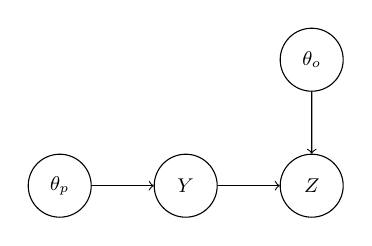
\begin{tikzpicture}[scale=0.8,every node/.style={transform shape}]
%[inner sep=1mm] 
[line width=1pt]
\path (0,0) node (thetap) [shape=circle,minimum size=1cm,draw] {\small $\theta_p$};
\path (2,0) node (y) [shape=circle,minimum size=1cm,draw] {\small $Y$};
\path (4,0) node (zo) [shape=circle,minimum size=1cm,draw] {\small $Z$};
\path (4,2) node (thetao) [shape=circle,minimum size=1cm,draw] {\small $\theta_o$};

\draw [->] (thetap) to (y);
\draw [->] (y) to (zo);
\draw [->] (thetao) to (zo);
\end{tikzpicture}
\end{figure}

\noindent %In this case no numerical model outputs are needed, as the prior process model $Y$ is deemed to be sufficiently representative such that simulator model outputs, which for now we can treat as realisations of some random process $Z_m$, would not provide any further information about the process model, i.e. $p(Y | \theta_p,Z_m) \approx p(Y | \theta_p)$. 

The object of interest in DA is the distribution of the field $Y$ given the prior scientific understanding (in this case the level 2 model) and observations, i.e.~$p(Y|Z)$. This is found by applying Bayes' Theorem and marginalising out the unknown parameters:
\begin{equation}
p(Y|Z) \propto \iint p(Z | Y, \theta_o)p(Y | \theta_p)p(\theta_o, \theta_p) \intd \theta_p \intd\theta_o.
\end{equation}

\noindent Unlike conventional assimilation methods, simulator outputs are not explicitly present within this framework. This class of approaches however still should be considered as a DA method as per the definition in Section 1. 

In the mechanistically motivated approach, an instance of \emph{science-based parameterization} \citep{Leeds_2012}, the numerical model is deemed to be faithful to the true process, and thus able to reproduce the emergent phenomena. This approach can thus only be used when there exists a model which is sufficiently simple and yet realistic enough to define the Level 2 process.  In \cite{Hooten_2008}, for example, the numerical model is Fisher's reaction-diffusion equation whilst the stochastic model is the finite-differenced, explicit Euler discrete equivalent. Similarly, a process model derived from heat equation is used for paleoclimate temperature reconstruction by \cite{Brynjarsdottir_2011}. In \cite{Wikle_2001}, the simplified model is the set of linear shallow-water equations subsequently reduced in dimensionality using an orthogonal basis set. In \cite{Berliner_2003b} air-sea interactions are studied through stochastic, simplified atmospheric and quasi-geostrophic ocean models. In \cite{Milliff_2011} a process model for the vector winds is based on approximations to the Rayleigh friction equation. In \cite{Cressie_2010} a multivariate linear dynamical system  is used to model the spatio-temporal progression of global aerosol levels.


In many cases a mechanistic-motivated model is not self-evident, particularly when what is termed the \lq process model\rq~is actually just one physical process influenced by several others within a complex network of models. In such cases no simple structure for $Y$ exists. The first alternative is a fully data-driven approach where numerical models are ignored entirely. The second, discussed next, is to integrate the (unsimplified) physical models directly.


\subsection{The simulator-informed prior}\label{sec:mip}

The simulator-informed prior approach is similar to the previous case, in that one attempts to configure the process model based on available science, with the difference that it is the numerical model outputs which are used to inform the process model $Y$: the numerical model \emph{structure} itself is not explicitly used.  Here, therefore, the process model in the hierarchial framework is one which is able to reconstruct the uncertainty of a physical (deterministic) simulator through uncertainties in simulator inputs and parameters, which could refer to anything from boundary conditions to forcings to solver resolution \citep{Goldstein_2009}. Loosely speaking, uncertainty is shifted from the governing \emph{structure} to the \emph{input parameters}. Structural discrepancy in this framework is sometimes still catered for through an added discrepancy term $\delta$, found by comparing the observations to the model outputs \citep{Kennedy_2001}.

Denote an imperfect simulator of $Y$ as $f(\vartheta_m)$, $\vartheta_m \in \Theta_m$. The process model $Y$ is then defined as the simulator evaluated at some (random) input $\theta_m \in \Theta_m$ with an added discrepancy $\delta$. It is important to render explicit the difference between (i) the variable $\vartheta_m$ which indexes $\Theta_m$ and (ii) $\theta_m$ which is a random variable over the same space. $f(\vartheta_m)$ is a deterministic function mapping $\Theta_m$ to $\mathcal{Y}$, whilst $f(\theta_m)$ is a transformation of a random variable and takes values in $\mathcal{Y}$, the distribution of which is fully governed by that of $\theta_m$ (the study of $f(\theta_m)$ is termed \emph{uncertainty analysis} by \cite{OHagan_1998}). For example, assume that $f(\vartheta_m)$ produces an air pollution map subject to a pollutant source location $\vartheta_m$. We can clearly produce as many maps as we wish to by perturbing $\vartheta_m$, and sometimes we want to model this relationship (see Emulation later), however the process $Y$ is defined to be $f(\cdot)$ evaluated at $\theta_m$, and we generally would also like to evaluate a posterior distribution over $\theta_m$ (termed Bayesian calibration by \cite{Kennedy_2001}). 

Returning to the process model, the inaccuracy in the simulator is compensated for with the use of a discrepancy term $\delta$ so that
\begin{equation}
Y = f(\theta_{m}) + \delta,
\end{equation}
\noindent which, if given as $\delta \sim \mathcal{N}(\mu_\delta,\Sigma_\delta)$, induces the conditional distribution 
\begin{equation}
p(Y | \theta_m, \theta_\delta) = \mathcal{N}(f(\theta_m) + \mu_\delta, \Sigma_\delta).
\end{equation}
\noindent The discrepancy term frequently plays a crucial role in the framework \citep{Brynjarsdottir_2013}. In general $\delta$ may also be dependent on $\theta_m$ and there are some ways, not reviewed here, to tackle this problem \citep[e.g.][Section 7.2]{Rougier_2007}. 
%It is important to stress the here $\theta^*$ is the unknown (we will place a prior over $\theta^*$) and $\theta_m$ should be treated as independent variables on an extended domain. The unknown appears in the constraint which is not standard. However 
%this equation leads to a simple conditional distribution if $y$ is a deterministic function of $\theta_m$ (i.e. $y$ is fully defined by $\theta_m$, as is the case with deterministic simulators) since then, for $\theta_m = \theta^*$ (and ignoring $\delta$ for the time being), $p(y | \theta^*) = \delta(y - y(\theta^*))$ so that 
%\begin{equation}
%p(y^* | \theta^*) = \int p(y^*|y)p(y | \theta^*) \intd y = p(y^* | y(\theta^*))
%\end{equation}
%\noindent which explicitly shows the relationship between $y^*$ and $\theta^*$ and is invariably a very complicated distribution. 
The ensuing graphical model for this setup is as follows
\begin{figure}[h!]
\centering
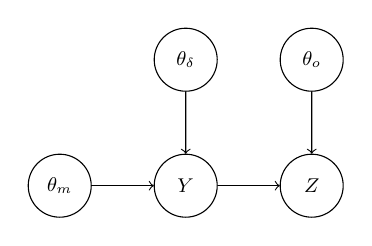
\begin{tikzpicture}[scale=0.8,every node/.style={transform shape}]
%[inner sep=1mm] 
[line width=1pt]
\path (2,0) node (thetam) [shape=circle,minimum size=1cm,draw] {\small $\theta_m$};
\path (4,0) node (ystar) [shape=circle,minimum size=1cm,draw] {\small $Y$};
\path (6,0) node (zo) [shape=circle,minimum size=1cm,draw] {\small $Z$};
\path (6,2) node (thetao) [shape=circle,minimum size=1cm,draw] {\small $\theta_o$};
\path (4,2) node (thetad) [shape=circle,minimum size=1cm,draw] {\small $\theta_\delta$};

\draw [->] (thetam) to (ystar);
\draw [->] (ystar) to (zo);
\draw [->] (thetao) to (zo);
\draw [->] (thetad) to (ystar);
\end{tikzpicture}
\end{figure}

\newpage
\noindent This is once again the 3-layer hierarchical model but with the unknown parameters $\theta_m$ actual input parameters to the deterministic model. The DA task of computing $p(Y | Z)$ is then carried out by marginalising out all the nuisance variables
\begin{equation}\label{eq:Sim_simple}
p(Y|Z) \propto \iiint p(Z | Y, \theta_o)p(Y |f(\theta_m), \theta_\delta)p(\theta_o, \theta_m, \theta_\delta) \intd \theta_m \intd\theta_o \intd\theta_\delta.
\end{equation}

The problem with this setup is that a typical Markov chain Monte Carlo (MCMC) scheme used to evaluate (\ref{eq:Sim_simple}) requires repeated evaluation of $f(\cdot)$, which is computationally expensive except for the rare case of a simple $f(\cdot)$ \citep{Higdon_2004}. %A discussion on (bad) choices for $p(\theta_m)$ are given in \cite[][Section 8.1]{Rougier_2007}.

A special case of the simulator-informed prior is the Ensemble Kalman Filter, in which the random parameters $\theta_m$ (usually taken to be initial conditions) are represented by an ensemble. Samples from the conditional distribution $p(Y | f(\theta_m),\theta_\delta)$ are then obtained by forward simulating the initial samples through $f(\cdot)$. Gaussian approximations are then used to render the update (\ref{eq:Sim_simple}) tractable \citep{Burgers_1998}. %For more details see Example 1 in Appendix A.


\subsubsection*{Emulation}

Emulation is an extension of the basic simulator-informed prior approach for when $f(\cdot)$ is too complex to evaluate repeatedly. In emulation we consider the presence of a secondary stochastic process $\widetilde{Y}$ which describes a simple probabilistic relationship between $\vartheta_m$ and $Y$. In particular, let $g(\cdot)$ denote a random function over the space $\Theta_m$. Then, if a simple linear relationship can be found for $\widetilde{Y}(\vartheta_i) = g(\vartheta_i;\theta_p)$, huge simplifications are possible. 

Formulating $\widetilde{Y}$ as a stochastic model over $\vartheta$ is a procedure known as \emph{emulation}. An emulator is typically constructed by taking $N$ design points $\{\vartheta_i\}_{i=1}^N$, running $f(\vartheta_i)$ for each $i$, and then treating each output as an `observation' of the simpler model $\widetilde{Y}$ with input parameters $\vartheta_i$. Note that an emulator provides no information whatsoever on the `true' input $\theta_m$, and should be merely regarded as a convenient way of exploring $\Theta_m$ without the computational burden of repeatedly evaluating $f(\cdot)$.

The model outputs themselves can be treated as (observed) instantiations of random processes $\{Y_m(\vartheta_i)\}$, which are simply $\widetilde{Y}(\vartheta_i)$ up to the aforementioned discrepancy term:

\begin{equation}
Y_{m,i} = \widetilde{Y}(\vartheta_i) + \delta \\
\end{equation}

\noindent For the simple linear case, this reduces to
\begin{equation}\label{eq:linear_emulator}
\widetilde{Y}(\vartheta_i) = \beta\vartheta_i + e_i, ~~~~~ e_i \sim \mathcal{N}(0,\sigma^2_e),
\end{equation}
\noindent where we collect the `process parameters' into $\theta_p = (\beta,\sigma^2_e)$.

From the outset, emulation tends to add complexity to the inferential problem, since we have introduced a second stochastic process. Indeed, the number of parameters increases with the use of an emulator, but this is generally a small price to pay for the reduction in computational effort. The effect of introducing an emulator is an added process layer resulting in the following extended hierarchical framework (dashed box encloses the emulator):

\begin{figure}[h!]
\centering
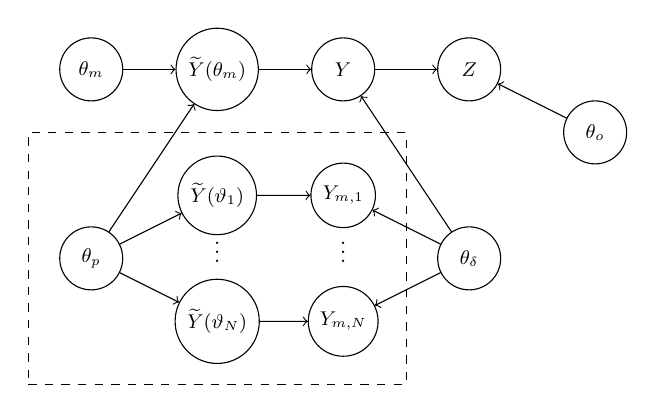
\begin{tikzpicture}[scale=0.8,every node/.style={transform shape}]
%[inner sep=1mm] 
[line width=1pt]
\path (6,0) node (zo) [shape=circle,minimum size=1cm,draw] {\small $Z$};
\path (8,-1) node (thetao) [shape=circle,minimum size=1cm,draw] {\small $\theta_o$};
\path (4,0) node (y) [shape=circle,minimum size=1cm,draw] {\small $Y$};
\path (2,0) node (yt) [shape=circle,minimum size=1cm,draw] {\small $\widetilde{Y}(\theta_m)$};
\path (0,0) node (thetam) [shape=circle,minimum size=1cm,draw] {\small $\theta_m$};

\path (4,-2) node (y1) [shape=circle,minimum size=1cm,draw] {\small $Y_{m,1}$};
\path (2,-2) node (yt1) [shape=circle,minimum size=1cm,draw] {\small $\widetilde{Y}(\vartheta_1)$};
\path (4,-4) node (y2) [shape=circle,minimum size=1cm,draw] {\small $Y_{m,N}$};
\path (2,-4) node (yt2) [shape=circle,minimum size=1cm,draw] {\small $\widetilde{Y}(\vartheta_N)$};
\path (2,-2.8) node (dots1){$\vdots$};
\path (4,-2.8) node (dots2){$\vdots$};

\path (6,-3) node (thetad) [shape=circle,minimum size=1cm,draw] {\small $\theta_\delta$};
\path (0,-3) node (thetap) [shape=circle,minimum size=1cm,draw] {\small $\theta_p$};

\draw [->] (thetap) to (yt1);
\draw [->] (thetap) to (yt2);
\draw [->] (thetap) to (yt);
\draw [->] (yt1) to (y1);
\draw [->] (yt2) to (y2);
\draw [->] (thetam) to (yt);
\draw [->] (yt) to (y);
\draw [->] (y) to (zo);
\draw [->] (thetao) to (zo);
\draw [->] (thetad) to (y);
\draw [->] (thetad) to (y1);
\draw [->] (thetad) to (y2);

\draw[dashed] (-1,-5) -- (5,-5) -- (5,-1) -- (-1,-1) -- (-1,-5);

\end{tikzpicture}
\end{figure}





The observations $Z$ are informative of $\theta_p$ and $\theta_\delta$, but in practice the emulator is constructed offline and plug-in estimates for $\theta_p$, say $\hat \theta_p$ are used. This approximation is valid when $Z$ is deemed to contain relatively little, if any, information on $\theta_p$ and $\theta_\delta$ and is appropriate in most scenarios. Considering the simple emulator of (\ref{eq:linear_emulator}), the offline setup would involve taking the $N$ inputs $\vartheta_i$, the $N$ outputs $y_{m,i}$ and finding estimates for $\beta$ and $\sigma^2_e$ using standard methods. Then the hierarchical model reduces to the following:

\begin{itemize}
\item Level 1: Observation model: $p(Z | Y, \theta_o)$
\item Level 2: Process model: $p(Y | \widetilde{Y}, \theta_\delta)$
\item Level 3: Emulator: $p(\widetilde{Y} | \theta_m; \hat\theta_p)$
\item Level 4: Parameter model: $p(\theta_o,\theta_\delta)$
\end{itemize}

The DA task is then completed as follows:
\begin{equation}\label{eq:Sim_simple2}
p(Y|Z) \propto \iiiint p(Z | Y, \theta_o)p(Y | \widetilde{Y},\theta_\delta)p(\widetilde{Y} | \theta_m; \hat\theta_p)p(\theta_o, \theta_\delta, \theta_m) \intd\theta_o. \intd\theta_\delta\intd\theta_m\intd\widetilde{Y}
\end{equation}


\noindent When comparing to (\ref{eq:Sim_simple}), we see that the use of an emulator introduces the term $p(\widetilde{Y} | \theta_m; \theta_p)$, a term which takes into account the simplified simulator output. Computational gains are achieved since sampling from $p(\widetilde{Y} | \theta_m; \hat\theta_p)$ is much cheaper than simulating from $f(\cdot)$. Note that the original simulator-informed prior can be achieved by replacing the emulator with the simulator, i.e.~simply by substituting $p(\widetilde{Y} | \theta_m) = \delta(\widetilde{Y} - f(\theta_m))$ in (\ref{eq:Sim_simple2}).
%
%
%\begin{equation}
%p(y^*|Z,z_m,\vartheta_m) \propto \iint p(Z | y^*, \theta_o)p(y^* | \theta_\delta, y,\theta_m)p(z_m | y)p(y | \theta_p,\vartheta_m)p(\theta^*,\theta_o, \theta_p, \theta_\delta) \intd \theta_p \intd\theta_o \intd\theta_\delta \intd\theta_m \intd y
%\end{equation}
%\noindent which, although is augmented with respect to (\ref{eq:Sim_simple}), is much easier to work with since both $p(y^* | \theta_\delta,y,\theta_m)$ and  $p(y | z_m,\theta_p,\vartheta_m) \propto p(z_m | y)p(y | \theta_p,\vartheta_m)$ are easy to evaluate up to a constant of proportionality (the latter intentionally being constructed to do so). The caveat is that now, conceptually, the framework is less straightforward. We have introduced a new set of unknowns ($\theta_p$) which typically configure the covariances defined on the domain of interest (including $\Theta_m$), and we have introduced an experimental design problem, where one needs to strategically compute a set of simulation runs $z_m = f(\vartheta_m)$ for various $\vartheta_m$ such that we have enough information to estimate $\theta_p$ and thus establish our belief on $f(\vartheta_m)$. 

In many cases, emulation is the only means with which to perform assimilation in real systems, particularly when the dimensionlity of $\theta_m$ is large. It has proved particularly useful in the environmental sciences, for example in the study of aerosol-cloud interactions \citep{Lee_2013}, ice-sheet dynamics \citep{Gladstone_2012, McNeall_2013}, marine ecosystems \citep{Leeds_2013} and climate change \citep{Holden_2013}.


The simulator-informed prior approach bears many similarities to the mechanistically motivated model mentioned previously. Arguably it is more faithful to the underlying science; in mechanistic models the original model parameters $\theta_m$ feature as process parameters $\theta_p$ but may significantly change in interpretation due to the simplifications and solver method adopted. With this latter approach we can fully retain the physical interpretation of the model parameters $\theta_m$, although we stress that due to the numerical model inadequacy or solver even these inputs need not even be physically plausible, let alone representative of some underlying truth \citep{Kennedy_2001}. However we can safely assume that they are more informative to scientists than what would typically constitute $\theta_p$ in a mechanistically-motivated approach. Note that although we have categorised the mechanistically motivated stochastic model and the simulator-informed prior approach separately, they can also be used within the same framework when multiple fields and data need to be assimilated simultaneously \citep{Pagendam_2014}. 

In both of the approaches described so far, the underlying science takes a central role either in the design or the estimation of the process. Next we consider the case where model outputs are considered as pure \lq observations\rq~ of the underlying process and where the science behind the model generated outputs takes a lesser role.

\subsection{The multi-observation approach}\label{sec:mo}

It is frequently the case that the numerical model which has generated the output is not of direct relevance to the assimilation problem. The task is, rather, to treat the model outputs $Y_m$ as surrogate observations in order to find optimal estimates for the true underlying process $Y$ under certain (often implicit) distributional assumptions \citep{Berliner_2012}. This method is referred to as the \lq data fusion\rq~method by \cite{Gelfand_2009}. The general hierarchical framework is
\begin{itemize}
\item Level 1a: Observation model: $p(Z | Y, \theta_o)$
\item Level 1b: Numerical model: $p(Y_m | Y, \theta_m)$
\item Level 2: Process model: $p(Y | \theta_p)$
\item Level 3: Parameter model: $p(\theta_o, \theta_p, \theta_m)$
\end{itemize}

A direct implementation of data fusion is given by \cite{Fuentes_2005} for modelling air pollution data in the US. The model outputs are assumed to be biased and scaled representations of the truth
\begin{equation}
Y_m = \delta_1 + \delta_2Y + e,
\end{equation}
\noindent while the observations are deemed unbiased. The process model is a Gaussian process (GP) with hyperparameters which need to be estimated from both the model and observation outputs. The graphical model for this type of assimilation is as follows:
\begin{figure}[h!]
\centering
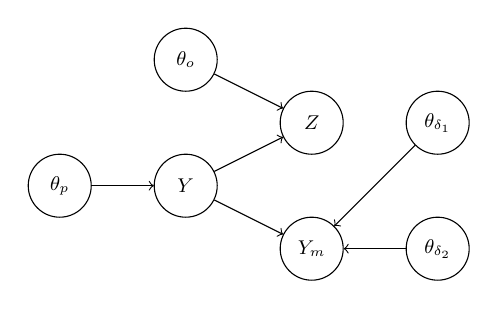
\begin{tikzpicture}[scale=0.8,every node/.style={transform shape}]
%[inner sep=1mm] 
[line width=1pt]
\path (2,0) node (thetap) [shape=circle,minimum size=1cm,draw] {\small $\theta_p$};
\path (4,0) node (ystar) [shape=circle,minimum size=1cm,draw] {\small $Y$};
\path (6,1) node (zo) [shape=circle,minimum size=1cm,draw] {\small $Z$};
\path (4,2) node (thetao) [shape=circle,minimum size=1cm,draw] {\small $\theta_o$};
\path (6,-1) node (zm) [shape=circle,minimum size=1cm,draw] {\small $Y_m$};
%\path (4,-2) node (thetam) [shape=circle,minimum size=1cm,draw] {\small $\theta_m$};
\path (8,1) node (thetad1) [shape=circle,minimum size=1cm,draw] {\small $\theta_{\delta_1}$};
\path (8,-1) node (thetad2) [shape=circle,minimum size=1cm,draw] {\small $\theta_{\delta_2}$};

\draw [->] (thetap) to (ystar);
\draw [->] (thetao) to (zo);
\draw [->] (ystar) to (zo);
\draw [->] (ystar) to (zm);
%\draw [->] (thetam) to (zm);
\draw [->] (thetad1) to (zm);
\draw [->] (thetad2) to (zm);
\end{tikzpicture}
\end{figure}

\noindent \cite{McMillan_2010} used an identical framework (albeit with inference at an aerial resolution and with no $\delta_2$), to combine data from monitoring sites with the Community Multi-scale Air Quality (CMAQ) model output to obtain estimates on PM$_{2.5}$ particulate matter. Here the process model was a generic, separable space-time model with spatial precision matrix given by the conditional auto-regressive(1) (AR1) model \citep{Rue_2005} and the temporal covariance by the AR1 process. A more elaborate version which facilitates inference at the point scale is given by \cite{Sahu_2010}. Multiple observation sources can be included, see for instance \cite{Smith_2007, Kang_2012}. 

The works mentioned so far all use black-box process models which are flexible so as to accommodate both the observed data and the model output. Mechanistically motivated models for $Y$, do however frequently appear in this context; for example in \cite{Milliff_2011} where scatterometer data ($Z$) is integrated with weather forecasts to obtain estimates of the surface-vector winds. Finally we note that in some cases, model outputs may be used to also induce secondary Level 2 process priors. In this case Bayesian melding \citep{Poole_2000} would be necessary to elicit a single process model prior.  


The multi-observation approach provide a neat way for assimilating multiple data sets (from models or/and observations) and is conceptually much simpler than the simulator-informed prior approach. One difficulty is that the relationship between $Y$ and $Y_m$ needs to be specified. One subtle, yet important advantage to the former approaches is that since the model output is expressed in terms of the process we can deal with problems such as change of support \citep{Wikle_2005} with ease (for example, we can say that the model output is an \emph{averaged} version of the true process). Methods in this category are fully focused on realisations and not on the tuning/calibration parameters used to generate the model outputs; these frequently do not feature at all.  


\section{Data-feature assimilation}\label{sec:data-feature}

All the above implicitly place considerable emphasis on either the numerical model structure (in the  case of mechanistically-motivated models) or the model output itself (in the case of the simulator-informed prior and the multi-observation approach). In fact, frequently observations are used to solely `correct' the model output, reflecting a pre-supposition that the outputs are mostly valid save for some minor descrepancy. At the other end of the spectrum, data-driven analysts implicitly assume that such is the abundance and coverage of data today (particularly from satellite instruments), numerical models need play a lesser role \citep[see][for a suite for such methods in a spatial context]{Bradley_2014}. 

However there are cases when data-driven approaches are not suitable, irrespective of data abundance. Consider, for example, the simple case when $Z$ records a linear combination of two, possibly interacting processes:
\begin{equation}\label{eq:problem}
Z = Y_1 + Y_2 + e.
\end{equation}

\noindent In this case the unobserved $Y_1$ and $Y_2$ are confounded \citep[when $Y_1$ and $Y_2$ are multi-variate Gaussian, (\ref{eq:problem}) is a saturated collection of co-linear relationships, see][]{Hodges_2010} and whatever the observation coverage, a posteriori these two fields are fully sensitive on our prior judments on $Y_1$ and $Y_2$. In this case one might argue that incorporating a simulator output to constrain at least one of the latent processes might be the best option for DA. However if the model output has substantial (unquantifiable) discrepancy, then this plug-in estimate might not be conducive to the assimilation task. It is unfortunately the case that models tend to perform unfavourably when they cannot be adequately validated, for example due to observation processes which take the form (\ref{eq:problem}) \citep{Zammit_2014}.

Frequently geoscientists themselves would be the first to acknowledge when and if simulator outputs are unreliable.  Nevertheless, even in this case there are aspects of simulator outputs which can be incorporated when the predominantly data-driven approach is a desirable course of action. In this section we consider such a suite of methods which are selective in their dependence on the underlying simulator, whilst not being as detached from the physical mechanisms as multi-observation approaches (Section \ref{sec:mo}) and not relying too heavily on the simulator outputs \emph{talis qualis} (Section \ref{sec:mip}). 

%There are cases where the latter would be counter-productive in assimilation: 
%\begin{enumerate}
%\item When the simulator output is either not reliable, or very hard to validate. This is, unfortunately, the case for natural processes which are also poorly observed such as solid-earth processes or those occurring in the deep ocean or in remote areas of the world such as Antarctica \citep{Guo_2012}. 
%\item When the numerical model contains several tuning parameters which are unidentifiable (cannot be calibrated). This is the case for example when treating surface mass balance anomalies in Antarctica, where the anomaly is taken with respect to a long-term \emph{balance state} which is unknown and in all probability highly unstructured spatially. 
%\end{enumerate}
%In both cases, frequently specialists themselves would be the first to acknowledge that the output and associated uncertainties could be highly inaccurate -- indeed in this case it is debatable whether a data assimilation procedure should at all be used and a data-driven solution might be the appropriate way forward for inference, unless we are faced with under-determined problems such as that discussed next. 

%\subsection{Source separation in environmental systems}\label{sec:sourcesep}
%
%For complex physical systems which we deal with, and in particular with interacting systems, fully data-driven approaches (using empirical methods or full Bayes) are not always possible. Consider for example the simple scenario
%\begin{equation}\label{eq:problem}
%Z = y_1 + y_2 + e
%\end{equation}
%\noindent where $Z$ are experimental observations and a priori $y_1,y_2 \sim \mathcal{N}(0,{\Sigma})$ and $e$ is uncorrelated white noise. Here the unobserved $y_1$ and $y_2$ are confounded (in fact (\ref{eq:problem}) is a saturated collection of co-linear relationships) and whatever the observation coverage, a posterior these two fields are fully sensitive on the prior. In this case one might argue that incorporating a numerical model output to set the prior on at least one of the latent processes might be the best option for data assimilation. However, using the above methods, models with potential substantial discrepancy might not be conducive to the inferential task. 
%
%The source separation problem is a natural generalization of the treatment of \cite{Hodges_2010} who considered the related model
%\begin{equation}\label{eq:problem2}
%\yvec = \beta \dvec + \xvec + \evec
%\end{equation}
%
%\noindent where $\beta$ is an unknown parameter, $\dvec$ is a fixed effect, $\xvec$ is the latent process and $\evec$ has precision $\tau\Imat$. In spatial applications, the precision matrix $\Qmat = \Sigma^{-1}$ is frequently sparse and neighbourhood dependent, so that $\xvec$ usually defines a Gaussian Markov Random Field (GMRF) or conditionally autoregressive prior. Degenerate $\Qmat$ is used for intrinsic versions, these will not be discussed here.  Unidentifiability of $\beta$ in this problem stems from co-linearity between $\dvec$ and the spectral components of $\xvec$, obtained through the decomposition $\Qmat = \Zmat \Lambda \Zmat^T$ where $\Zmat$ is the eigenvector matrix and $\Lambda$ is diagonal with elements corresponding to the eigenvalues of $\Qmat$. The equivalent model
%\begin{equation}
%\yvec = \beta \dvec + \Zmat \bvec + \evec
%\end{equation}
%has an implicit prior on $\bvec$ centred on zero with variances inversely proportional to the eigenvalues $\Lambda$. Higher variances would be attributed to the lower frequency components, whilst lower variances (smaller orders of magnitude) with the higher frequencies. Colinaerity between $\dvec$ and columns of $\Zmat$ can drastically (adversely) alter the posterior estimate of $\beta$, both in mean and variance. 
%
%Consider again (\ref{eq:problem}). Now $\yvec  = \Zmat_1 \bvec_1 + \Zmat_2 \bvec_2 + \evec$ where we have assumed that $\xvec_1$ and $\xvec_2$ have different prior distributional properties. It is interesting to see how the Bayes update behaves in this case. For simplicity assume that $\Zmat_1 \equiv \Zmat_2 = \Zmat$ (for practical purposes, highly co-linear) but that $\Lambda_1 \ne \Lambda_2$, then it can be shown that 
%\begin{equation}
%var(b^i_1 | \yvec) = \frac{\lambda^i_2 + \tau}{\lambda^i_1\lambda^i_2 + \tau(\lambda^i_1 + \lambda^i_2)} 
%%\expect[b^i_1 | \yvec]/\expect[b^i_2 | \yvec] =\frac{\lambda^i_2 + \tau(1 - v^i)}{\lambda^i_1 + \tau(1- v^i)}
%\end{equation}
%\noindent which, under the prior assumption of spectral similarity ($\lambda^i_1 \equiv \lambda^i_2 = \lambda^i$) will have a lower-bound ($\tau \gg \lambda^i$) of $1/2\lambda^i$. This will not result in informative assessments on the marginals, in general, unless highly informative priors are set on both fields. Thus one would wish the spectral properties to differ a priori. For instance, by setting $\lambda_2^i \gg \lambda_1^i$, the lowerbound is given by the first term on the RHS in
%\begin{equation}
%var(b^i_1 | \yvec) = \frac{1}{\lambda^i_1 + \tau} + O(1/\lambda_2^i)
%\end{equation}
%\noindent which is also the standard Gaussian update in the absence of confounded fields. 
%
%It is therefore desirable to have prior distributions for $\xvec_1$ and $\xvec_2$ which have dissimilar spectral properties, a task which may be aided with simulator outputs. Selectively setting spectral properties corresponds to strategically choosing a set of constraints from simulator data using the four strategies outlined in Sections 3.3--3.6. 
%
%%Data-feature assimilation provides an all-important strategy in setting our prior spectral characteristics and thus aid uncertainty reduction on the posterior estimates. 




%In this work we show how to use other aspects of the numerical model within the framework, namely by specifying a Level 3 model on selected components from the simulator outputs which define \emph{features} deemed representative by the specialist. Despite its potential, this type of assimilation is remarkably rare in the environmental literature, although there are some isolated works which we will refer to throughout the ensuing discussion.

\subsection{Model setup}

From now on we shall assume a spatial domain of interest $\mathcal{O} \subset \mathbb{R}^d, d \ge 2$ indexed by $\svec$. Denote the process as  $Y(\svec): \mathbb{R}^d \rightarrow \mathbb{R}$. Under the assumption of observations with normally distributed errors, our Level 1 observation model is 
\begin{equation}
Z(\svec_i) = Y(\svec_i) + e_{o,i}, ~~~~ i = 1\dots m
\end{equation}
\noindent where $e_{o,i}$ is uncorrelated white noise with precision $\theta_o$ and $m$ is the number of observations. Note that $Y(\svec_i)$ need not be Gaussian, in general, although this is assumed throughout. Then $\Yvec = [Y(\svec_i), Y(\svec_2), \dots, Y(\svec_m)]$ is the record of physical observations. 

%Consider now a simulator $f(\svec,\varthetab_m)$. Then, we recall that the basic model-informed prior approach is to let
%\begin{equation}
%y^*(\svec_i) = f(\svec_i;\thetab_m) + \delta(\svec_i) + e_{y,i}, ~~~~ i = 1\dots m
%\end{equation}
%\noindent where $\delta(\svec_i)$ is a discrepancy term. $\delta(\svec)$ needs to be modelled itself, and frequently insight of what constitutes $\delta(\svec)$ needs to known and included appropriately. In this section we are concerned with cases where  either $\delta(\svec)$ is hard to construct from the available simulator outputs, or else too flexible for $f(\svec_i,\thetab_m)$ to impart knowledge on $ y(\svec_i)$ with the number of observations available. 
%
%The approach is similar to the use of the discrepancy in that we assume that the model output is spatially biased from the truth in some way. However we do not enforce a prior model on $\delta(\svec)$. 
%The approach rests on constructing two prior process distributions, one for the true process $Y(\svec)$ and one for the model outputs which share only some of the underlying parameters. As we shall see this is a very flexible framework and is ideal when the discrepancy is highly unstructured (or unknown) and only certain output features of the numerical model are deemed correct. The basic premise is to represent the true field, and that generated by simulators by stochastic models which share commonalities on a subset of their hyper-parameters (resulting in a selective borrowing of strength). In a Gaussian setting, the model is as follows

The basic premise of the approach is to construct two prior process distributions, one for the true process $Y(\svec)$ and one for the simulated process $\widetilde{Y}(\svec)$, which have only some of the underlying parameters in common. The partial sharing of underlying parameters results in a \emph{selective} borrowing of strength. The hierarchical model is as follows:

\begin{align}
Z(\svec_i) &\sim \mathcal{N}( Y(\svec_i),\theta_o^{-1}), \\
Y(\svec) &\sim \mathcal{GP}(\mu(\svec;\theta_p, \theta_c), k(\svec,\rvec;\theta_p, \theta_c)), \\
\widetilde{Y}(\svec) &\sim \mathcal{GP}(\mu(\svec;\tilde\theta_p, \theta_c), k(\svec,\rvec;\tilde\theta_p, \theta_c)), 
\end{align}

\noindent where $\mathcal{GP}(\mu(\svec),k(\svec,\rvec))$ denotes a Gaussian process on $\svec$ with mean $\mu(\svec)$ and covariance function $k(\svec,\rvec)$. The graphical model is

\begin{figure}[h!]
\centering
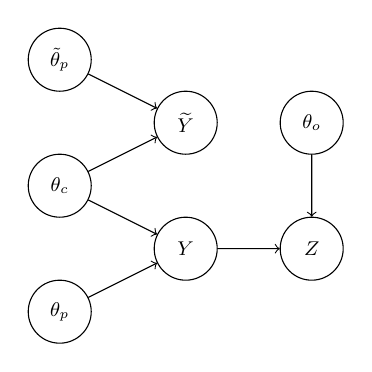
\begin{tikzpicture}[scale=0.8,every node/.style={transform shape}]
%[inner sep=1mm] 
[line width=1pt]
\path (2,4) node (gammam) [shape=circle,minimum size=1cm,draw] {\small $\tilde\theta_p$};
\path (2,0) node (gammat) [shape=circle,minimum size=1cm,draw] {\small $\theta_p$};
\path (2,2) node (gammac) [shape=circle,minimum size=1cm,draw] {\small $\theta_c$};
\path (4,3) node (y) [shape=circle,minimum size=1cm,draw] {\small $\widetilde{Y}$};
\path (4,1) node (ystar) [shape=circle,minimum size=1cm,draw] {\small $Y$};
\path (6,1) node (zo) [shape=circle,minimum size=1cm,draw] {\small $Z$};
\path (6,3) node (thetao) [shape=circle,minimum size=1cm,draw] {\small $\theta_o$};

\draw [->] (gammam) to (y);
\draw [->] (gammac) to (y);
\draw [->] (gammac) to (ystar);
\draw [->] (gammat) to (ystar);
\draw [->] (ystar) to (zo);
\draw [->] (thetao) to (zo);
\end{tikzpicture}
\end{figure}

\noindent $\tilde\theta_p$ are parameters which are believed to be \lq wrong\rq~in the sense that, a priori, they impart information on $\widetilde{Y}$ which is not considered valid for the true process $Y$. $\theta_p$ are the \lq true\rq~version of $\tilde\theta_p$ and $\theta_c$ are parameters believed to be common to both models. In terms of data-feature assimilation,  $\tilde\theta_p, \theta_c$ and $\theta_p$ describe the discarded, common and data-driven features respectively. In the following we provide some examples which motivate this hybrid approach.

%There are subtle yet significant differences to when a stochastic model (or a set of) are used to characterise $y(\svec,\varthetab)$ and $\delta(\svec)$ separately. First, unlike e.g. \cite{Higdon_2004}, we do not necessarily need to assume that all hyper-parameters of $\mathcal{GP}_2$ are representative of the truth. Further, we are not concerned with retaining dependency on $\varthetab$ as the complex nature of $\delta(\svec)$ is such that the model output, in the cases we are interested in, is itself not of use. The variability of the features in $\gammab_m$ which arise due to uncertainty in the parameters could be informative however.  Finally, the primary purpose of the exercise is assimilation and not prediction, obviating the need for a reliable parameter model and an estimate of the best parameter $\thetab_m$. 


% Note, however, that we do not constrain RP to be a Gaussian process as there are several interesting cases when this need not be the case. 

\subsection{Incorporation of spectral features}

First we consider the case when the scientist expresses confidence on the spectral composition of the simulator outputs, but not on the output values themselves. This is the case, for instance, when models are still in their early stage of development, or when there is a discrepancy term which is spatially varying and cannot be observed (e.g.~a long-term average). One possible model which captures this lack of understanding or confidence in the model outputs is as follows:

\begin{align}
Y(\svec) &= \Xmat(\svec)^T\betab + \upsilon(\svec; \gammab_c), \\
\widetilde{Y}(\svec) &= \Xmat(\svec)^T\tilde\betab + \tilde\upsilon(\svec; \gammab_c), \\
\upsilon, \tilde\upsilon &\stackrel{iid}{\sim} \mathcal{GP}(0,k(\svec,\rvec;\gammab_c)),
\end{align}

\noindent where $\betab, \tilde\betab$ weight some spatial regressors $\Xmat(\svec)$ and $\gammab_c$ are parameters appearing in the covariance function $k$. Note the subscripts employed: We are assuming that the numerical models are not informative of $\betab$, nor of the small-scale variation term $\upsilon$, but of the spectral composition of $\upsilon$. Following detrending of $Y(\svec)$, this scenario equates to using model outputs to help configure spectral filters which to use on the observed data. To see this assume that we have set $k(\svec,\rvec)$ to be the Mat{\'e}rn function of the form
\begin{equation}\label{eq:Matern}
k(\svec,\rvec) = \frac{\sigma^2}{2^{\nu-1}\Gamma(\nu)}(\kappa\| \svec - \rvec \|)K_\nu(\kappa\| \svec - \rvec \|),
\end{equation}
%In a data-driven setting one might first obtain point estimates for $\nu, \sigma^2$ and $\kappa$. 
\noindent where $\sigma^2$, $\kappa$ and $\nu$ are free parameters. By the auto-covariance theorem, which states that the Fourier transform of the auto-covariance function of the GP is the power spectral density of the signal, this is an implicit representation of the signal spectral characteristics. For the Mat{\'e}rn, the spectral density is 
\begin{equation}
R(\kvec) \propto (2\pi)^{-d}(\kappa^2 + ||\kvec||^2)^{-\alpha}, ~~~ \alpha = \nu + d/2,
\end{equation}
\noindent where $\kvec$ is the wavenumber and $d$ is the spatial dimensionality. Hence, by setting $\theta_c = \gammab_c = \{\nu, \sigma, \kappa\}$ we are asserting that the spectral composition of $\tilde\upsilon$ is the same as that for $\upsilon$. This assertion is warranted when a predominantly data-driven approach is desirable and only spatially sparse observations are available. 
%Note that we are not informing the prior mean of $Y(\svec)$ through the model outputs as is implicitly done when treating the model output as another data source.

%For illustration of this approach we generate two realizations from a Gaussian process and treat one as the real system and one as the model output. We then generate 10 equally spaced observations with standard deviation $\sigma = 0.5$ and estimate the hyperparameters (using a simple grid search in this problem) for the three options $\nu \in \{ 1/2, 3/2, 5/2\}$. For the problem in Fig. \ref{fig:GPtests} these are estimated as $\hat\nu = 5/2, \hat\sigma = 2.26, \hat \kappa = 0.26$ (the true values were $\hat\nu = 1/2, \sigma = 2, \hat \kappa = 0.1$). Note how the regressed curve (and associated uncertainty intervals) are overly smooth, and fails to capture variability of the true process. This would not be picked up using standard cross-validation techniques if our problem was defined by (\ref{eq:problem}).  We next re-do the exercise by first tuning the hyper-parameters based on the numerical model output. This now gives $\hat\nu = 1/2, \hat\sigma = 1.34, \hat \kappa = 0.31$. Note how the uncertainty intervals are now widened to cater for the lack of smoothness. The frequency-response estimated from the data and that from the numerical model are shown in Fig. \ref{fig:GPtests} together with that of the true process.
%
%\begin{figure*}[t!]
%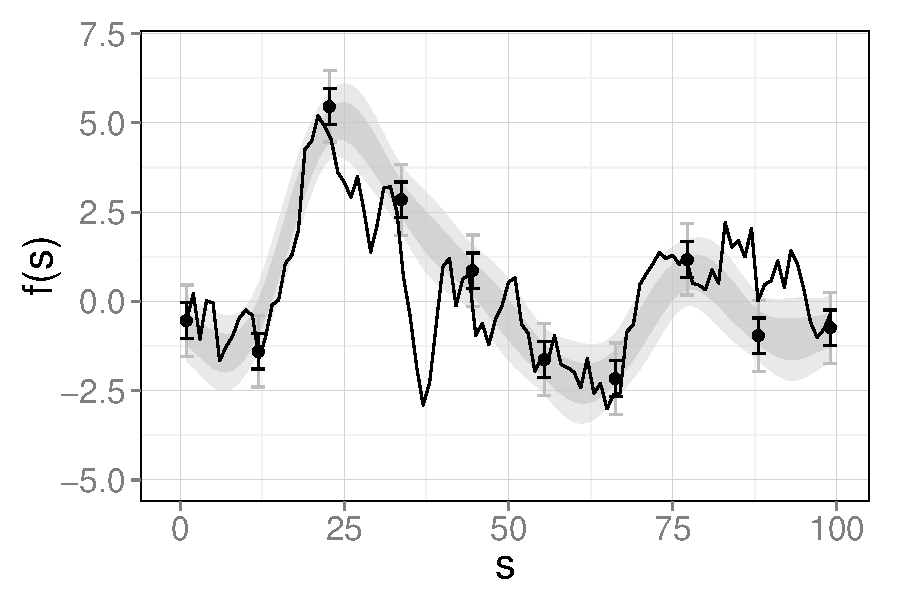
\includegraphics[width=2.8in]{GP1.pdf}
%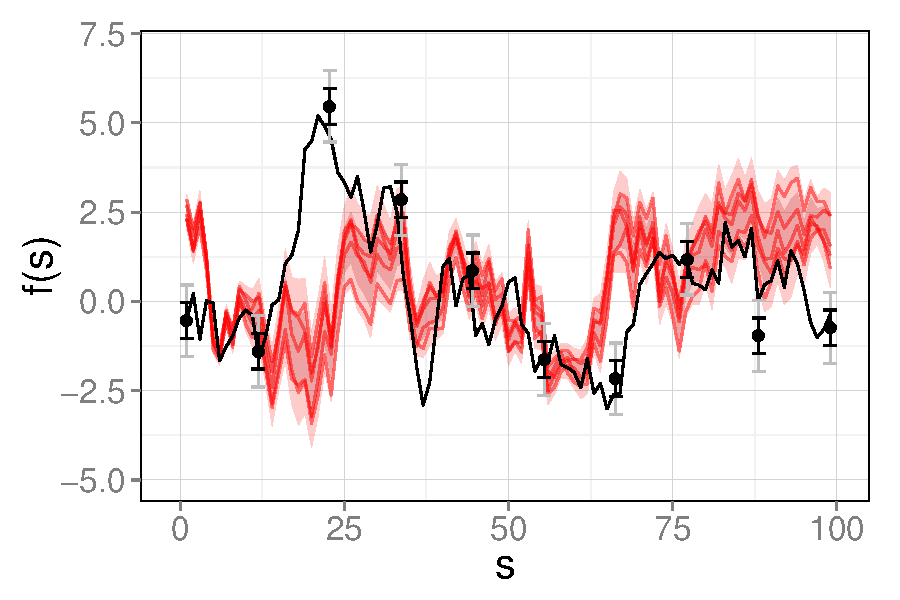
\includegraphics[width=2.8in]{GP2.pdf} \\
%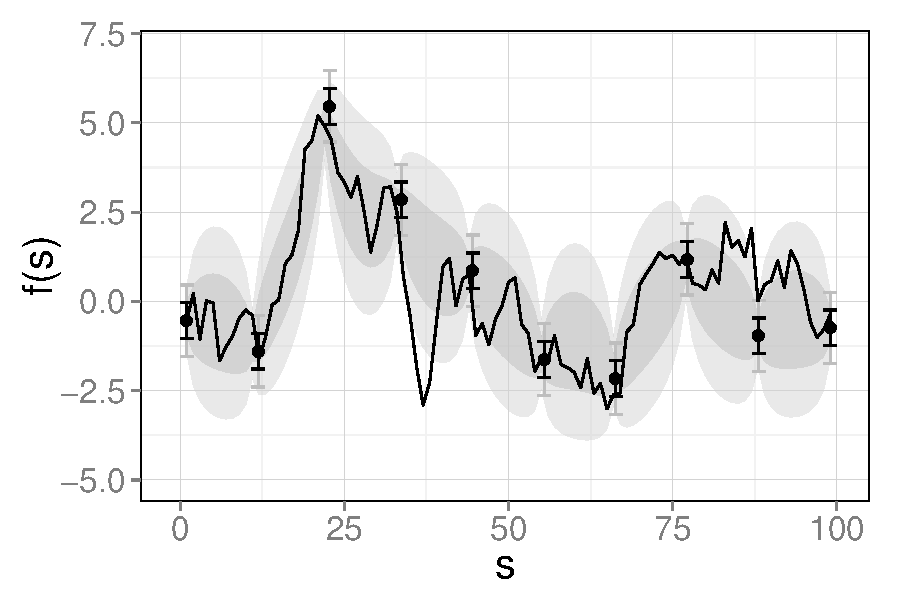
\includegraphics[width=2.8in]{GP3.pdf}
%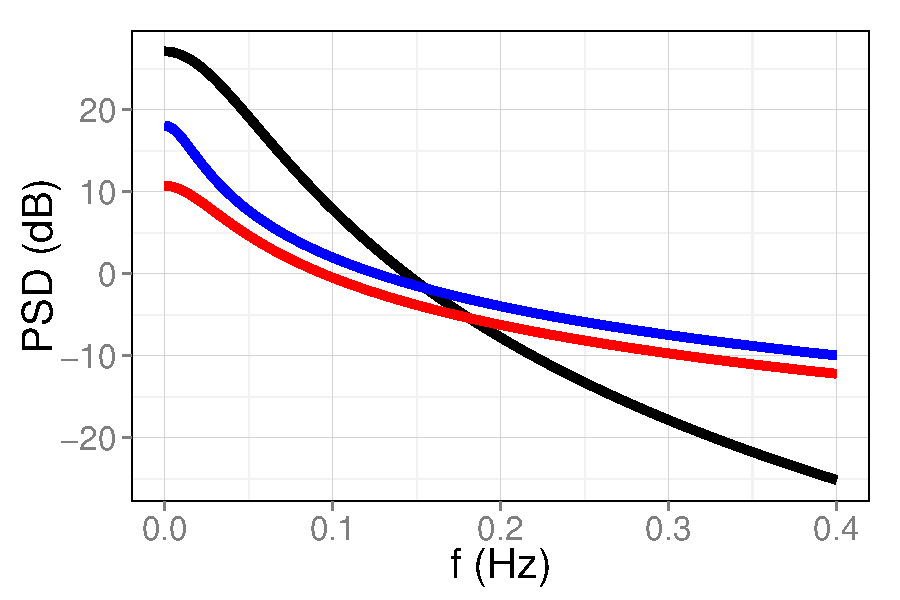
\includegraphics[width=2.8in]{GP4.pdf}
%\caption{Top left: Inference using empirical estimates of $\gamma_c$ from the data. Bottom left:  Inference using empirical estimates of $\gamma_c$ from model outputs. Top right: Truth (solid line), observations (dots with 1$\sigma$ and 2$\sigma$ error bars) and model simulations (red). Bottom right: True power spectrum (solid), power spectrum estmimated from the data (dotted) and from the model (dashed). Note how the high frequencies are under-represented in the data spectrum due to aliasing.}\label{fig:GPtests}
%\end{figure*}

Examples of works employing this approach include \cite{Berliner_2000} where the spatial covariance matrix of global mean temperature was estimated from surrogate model output, and \cite{Zammit_2014} where the heterogeneous characteristics of a precipitation anomaly were extracted from numerical model output and used to set up a prior spatial model. In the latter example, this approach proved invaluable in tackling the source separation problem in (\ref{eq:problem}).


\subsection{Incorporation of dynamical features}\label{sec:dynamical}

Spatio-temporal modelling is a powerful tool extensively employed in environmental applications such as air pollution monitoring \citep{Cameletti_2013, Sahu_2005}. Frequently, as in the fixed rank filtering case studies of \cite{Cressie_2010} and \cite{Kang_2010}, dynamic information may be obtained directly from the data \citep[see also][]{Wikle_2002,Dewar_2009}. In other cases this is not plausible, particularly when the observations are \lq patchy\rq~or are highly irregular in space and time. One way to overcome this problem is to extract dynamic information from the model output and using this to inform the dynamics the true process model $Y_k(\svec)$ where $k$ denotes the (discrete) temporal index. For a linear Gaussian spatio-temporal system the model employed is as follows:
\begin{align}
Y_{k+1}(\svec) &= [\mathcal{A};\theta_c]Y_k(\svec) + w_k(\svec;\theta_p), \\
\widetilde{Y}_{k+1}(\svec) &= [\mathcal{A};\theta_c]\widetilde{Y}_{k}(\svec) + \tilde w_{k}(\svec;\tilde\theta_p), 
\end{align}

\noindent where $\mathcal{A}$ is an operator propagating $Y_k(\svec)$ in time and $w_k(\svec)$ is an additive disturbance. This was the approach taken by \cite{Calder_2011} in modelling the spatio-temporal dynamics of aerosols where $\mathcal{A}$ was the integro-difference operator \citep{Kot_1986} and $\theta_c$ denoted the (spatially-varying) characteristics of flow direction and dispersion. The dynamic parameters describing the aerosol transportation patterns were estimated empirically offline, and then plugged into the model for $Y_{k+1}(\svec)$. This assumption is valid when the posterior variability on the parameters is small enough to be considered negligible \citep{Zammit_2014b}.

\subsection{Incorporation of spatial features (fingerprinting)}

In other cases one wishes to assimilate data with solely the spatial pattern of the simulator output, by which we mean a component function $\phi(\svec)$ which explains a substantial amount of variation in the output (e.g.~the first empirical orthogonal function following a decomposition of several simulations from $f(\cdot)$). This bears similarity to the use of empirical orthogonal functions derived from the data itself \citep[e.g.][]{Wikle_1999} as basis functions for dimensionality reduction of $Y$. In this case the simulator is taking the role of basis function construction. The following model is implied
\begin{align}
Y(\svec) &= \phi(\svec ; \theta_c) \beta + \upsilon(\svec;\theta_p), \\
\widetilde Y(\svec) &= \phi(\svec ; \theta_c) \tilde\beta + \tilde\upsilon(\svec;\tilde\theta_p),
\end{align}
\noindent where the parameters $\theta_c$ appear in a parametric representation of $\phi$. This is a natural approach to DA, however the most common appearance of this model is in a related technique known as \emph{fingerprinting}. In fingerprinting, the `fingerprint' $\phi(\svec; \theta_c)$ is generally deemed to be fully determined by $\widetilde Y$: as in Section \ref{sec:dynamical}, $\theta_c$ is estimated offline and then plugged into the model for $Y$. Then, a posterior distribution for $\beta$ concentrated around 0 is an indication that the simulator fingerprint is not apparent in the data. This approach was adopted by \cite{Berliner_2000} where the fingerprint used was a simulated temperature anomaly resulting from imposed $CO_2$ forcings. In the treatment \cite{Berliner_2000} suggest placing some prior judgments on $\theta_c$ as a possible modelling choice, in which case the data will be assumed to be informative of $\phi(\svec)$.

Others employing this approach include \cite{Wikle_2001}, where eigenvectors are estimated from a model describing sea-level pressure, the weights of which are subsequently estimated in assimilation. Constraining the process to lie on a low-dimensional space motivated by simulator output is beneficial when the observations are sparse, and is another approach to solving the confounding problem illustrated in (\ref{eq:problem}).

%\subsection{Incorporation of soft constraints}
%
%\red{Botond, can you also write this out and put in maybe a toy study from what you had in NIPS.}
%
%
%
%
%								
%
%
%\section{Conclusion}
%
%This article summarised the four main approaches to assimilating data with prior belief obtained from numerical model output. Such approaches are used to deal with the vast amount of information available to the statistician today, and selectively incorporate aspects of physical systems which corroborate expert judgment.These methods, and particularly those outlined in Section \ref{sec:data-feature} will play a major role in the modelling and inference of multi-variate (possibly under-determined) physical processes for the foreseeable future.

\bibliography{Assim_bib}

\newpage

\appendix            
\section{Examples}

\paragraph{Example 1: Ensemble Kalman Filtering}
Ensemble Kalman filtering (EnKF) is the simplest application of the simulator-informed prior approach approach where $\theta_m$ are the initial conditions at a given time (say $t$). The model ensemble is generated by running the simulator $f(\cdot)$ for a short time period until the next observation at $t+\Delta_t$ for each of the different initial conditions. In EnKF there is no discrepancy term, and all parameters (except $\theta_m$) are assumed known. This implies a one-to-one mapping between $\theta_m$ and $Y$ so that one of these terms (we choose $\theta_m$) can be omitted in a much simplified graphical model:
\begin{figure}[h!]
\centering
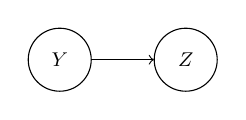
\begin{tikzpicture}[scale=0.8,every node/.style={transform shape}]
[inner sep=1mm] 
[line width=1pt]
\path (4,0) node (ystar) [shape=circle,minimum size=1cm,draw] {\small $Y$};
\path (6,0) node (zo) [shape=circle,minimum size=1cm,draw] {\small $Z$};
\draw [->] (ystar) to (zo);
\end{tikzpicture}
\end{figure}

\noindent The distribution of the true process $Y$ is fully determined by that of $\theta_m \sim p_{\theta_m}(\theta_m)$, and is given by
\begin{equation}
p(Y) = p_{\theta_m}(f^{-1}(Y))\left| \frac{\intd f^{-1}(Y)}{\intd Y}\right|
\end{equation}
\noindent Equation (\ref{eq:Sim_simple}) reduces to
\begin{equation}
p(Y|Z) \propto  p(Z | Y)p(Y)
\end{equation}
\noindent As earlier we are faced with a very complicated induced distribution due to presence of $f$ which, even if known, need not be invertible. In EnKF the computation is facilitated by approximating the induced distribution as a normal distribution
\begin{equation}
Y \sim \mathcal{N}(\mu_m,\Sigma_m; \theta_m)
\end{equation}
\noindent and $\mu_m = \expect[f(\theta_m)]$ and $\Sigma_m = var[f(\theta_m]$ which can be easily found empirically from a small ensemble of, say, 50 runs (details are given later).  

The \lq Kalman filtering\rq~in EnKF refers to the linear, sequential nature of this estimate i.e. $Z = CY + e$ with $e$ zero-mean Gaussian with covariance $\Sigma_o$ assumed.  The required posterior distribution is then
\begin{equation}
  p(Y | Z) \propto \exp\left(-\frac{1}{2}(Z - CY)^T\Sigma_o^{-1}(Z - CY) - \frac{1}{2}(Y - \mu_m)^T\Sigma_m^{-1}(Y - \mu_m) \right) 
\end{equation}
\noindent which is normally distributed with precision and mean given by
\begin{align}
\Sigma_a^{-1} &= C^T\Sigma_o^{-1}C + \Sigma_m^{-1} \\
\mu_a &= \Sigma_a[C^T\Sigma_o^{-1}Z + \Sigma^{-1}_m\mu_m]
\end{align}
\noindent The usual KF equations are obtained by applying the Sherman-Woodbury formula to the precision matrix to yield
\begin{align}
\Sigma_a &= (I - KC)\Sigma_m \\
\mu_a &= \mu_m + K(Z - C\mu_m) \label{eq:EnKFmean}
\end{align}
\noindent where $K = \Sigma_mC^T(\Sigma_o + C\Sigma_mC^T)^{-1}$ is the Kalman gain. Note that for the single model output case (where $\Sigma_f$ needs to be specified using some other means), $\mu_a$ reduces to the 3DVAR estimate \citep{Hamill_2000}.

The \lq Ensemble\rq~ in EnKF refers to the Monte Carlo nature alluded to earlier by which the mean and covariance are computed for when $f(\thetab_m) \in \mathbb{R}^{n \times N}$, where $N$ is the number of model ensembles and $n$ is the state dimensionality (i.e. $\thetab_m$ are $N$ samples from $p(\theta_m)$). The predictive mean is simply $\mu_m = \expect[f(\thetab_m)]$ while the covariance $\Sigma_m$ is estimated as the empirical covariance between the ensemble members as  $\Sigma_m = \expect[(f(\thetab_m) - \expect[f(\thetab_m)])(f(\thetab_m) - \expect[\thetab_m])^T]$. 

The update step is also carried out using these realisations, First an ensemble of pseudo-observations $z_{o,m} \in \mathbb{R}^{m \times N}$ is generated by repeatedly sampling from $\mathcal{N}(Z,\Sigma_o)$. Then the update (computation of posterior mean) is performed on each member separately to get a set of ensemble means $\mu_{a,m} \in \mathbb{R}^{n \times N}$ referred to as the \emph{analysed estimates}:
\begin{equation}
\mu_{a,m} = f(\thetab_m) + K(z_{o,m} - Cz_m)
\end{equation}
It can be shown that the mean of these estimates, $\expect[\mu_{a,m}]$, converges to $\mu_a$ in the large sample limit, as does the sample posterior covariance $\expect[(\mu_{a,m} - \expect[\mu_{a,m}])(\mu_{a,m} - \expect[\mu_{a,m}])^T]$ to the true posterior covariance $\Sigma_a$, see \cite{Burgers_1998} for further details.

EnKF is a quick and efficient way for DA. However simulation with $f(\cdot)$ needs to be quick and moreover, the assumptions imposed are strong: $p(y^* | Z)$ is restricted to be Gaussian (only the mean and covariance of the ensemble members are used), the observation models are linear and the posterior mean is effectively a weighted average of the model outputs and the observations. Full-blown sequential Monte Carlo (SMC) methods may be used to remedy this, however computational issues and degeneracy in high dimensional systems would be problematic. Model bias/discrepancy is not accounted for. Thus EnKF (or any corresponding SMC method) should only be used when the simulator $f(\cdot)$ is reliable, i.e. when observations are sufficiently regular in time so that any disrepancy arising due to $f(\cdot)$ may be safely assumed to be inconsequential.

\paragraph{Example 2: The linear Gaussian emulator} Here we consider a similar case to \cite{Higdon_2004} where $\theta_o$ is known. However to make the example even simpler we assume an emulator which is linear in $\vartheta_m$ and a model output (and hence observation) which is a scalar. For this example we will use bold typeface to denote vectors for clarity. Assume that we have $N$ runs of the full system with inputs $\varthetab_m$ and outputs $\zvec_m$. The full system equations are as follows:
\begin{align}
\zvec_o &= \yvec^* + \evec_o,~~~~ \evec_o \sim \mathcal{N}(0,\Sigma_o) \\
y^* &= y(\theta_m) + \delta,~~~~ \delta \sim \mathcal{N}(\mu_\delta,\sigma^2_\delta) \\
y(\vartheta_m) &= \beta\vartheta_m + e_y,~~~~ e_y \sim \mathcal{GP}(0,k(\vartheta_m,\vartheta_m';\theta_p')) \\
\zvec_m &= y(\varthetab_m) + \evec_m, ~~~~ \evec_m \sim \mathcal{N}(0,\Sigma_m)
\end{align}
\noindent where we let $\theta_\delta = (\mu_\delta,\sigma^2_\delta)$, $\theta_p = (\beta,\theta_p')$ and assume that $\theta_p'$ is independent of $\vartheta_m$ although this can be relaxed in practice (for example the variance is linearly related to $\vartheta_m$). The quantity $\Sigma_m$ is typically diagonal and reflects the small-scale error in emulator construction (also the nugget effect in kriging). The model outputs act as training data; the corresponding process values at $\varthetab_m$ are $\yvec = y(\varthetab_m)$. 

In this first stage it is required to find the posterior distribution of $y$ at a particular point $y(\theta_m)$, this is a classical problem in Gaussian process prediction \citep{Rasmussen_2006}. A trick to simplify computations in GP prediction is to directly consider the \emph{joint} distribution
\begin{equation}
p(\zvec_m,y^* | \theta_m,\varthetab_m) \propto \int p(\zvec_m,y^* | \yvec, \theta_m,\theta_\delta)p(\yvec | \varthetab_m,\theta_p)p(\theta_p) \intd \theta_p \intd \theta_\delta\intd \yvec
\end{equation}
\noindent If we can somehow fix $\theta_p,\theta_\delta$ (using, for instance empirical methods such as trend analysis and semivariograms, or at each sample in an MCMC scheme), then this distribution reduces to
\begin{equation}
p(\zvec_m,y^* | \theta_m,\varthetab_m) \propto \mathcal{N}\left(\begin{bmatrix}\beta\varthetab_m \\ \beta\theta_m + \mu_\delta \end{bmatrix},\begin{bmatrix} \Sigma_m + \Sigma_{\varthetab_m} & \Sigma_{\varthetab_m\theta_m} \\ \Sigma_{\theta_m\varthetab_m} & \sigma^2_{\theta_m} + \sigma^2_\delta \end{bmatrix}  \right)
\end{equation}
\noindent where $\Sigma_{\varthetab_m} = k(\varthetab_m,\varthetab_m)$ and $\Sigma_{\varthetab_m\theta_m} = k(\varthetab_m,\theta_m)$. By Gaussian conditioning we can then find $p(y^* | \zvec_m,\theta_m,\varthetab_m)$ as 
\begin{align}
p(y^* | \zvec_m,\theta_m,\varthetab_m) = \mathcal{N}(\Sigma_{\theta_m\varthetab_m}[\Sigma_{\varthetab_m\varthetab_m} &+ \Sigma_m]^{-1}(\zvec_m - \beta \varthetab_m) , \\
&\Sigma_{\theta_m\theta_m} - \Sigma_{\theta_m\varthetab_m}[\Sigma_{\varthetab_m\varthetab_m} + \Sigma_m]^{-1}\Sigma_{\varthetab_m\theta_m})
\end{align}
\noindent The next stage is to find $p(y^* | \zvec_o, \zvec_m, \theta_m, \varthetab_m) \propto p(\zvec_o | y^*)p(y^* | \zvec_m,\theta_m,\varthetab_m)$, a simple Guassian update which also results in closed form expressions for a given $\theta_m$. Now all that remains is to marginalise out $\theta_m$ which, even in this simplest of cases, will require sampling due to the complicated nature with which this variable appears in the problem (in machine learning terms, as a random  \emph{test point}). However sampling this posterior is very quick, unlike in the former case when $f(\vartheta_m)$ is repeatedly evaluated. In this case the effective dimensionality is only as large as the dimensionality of $\theta_m$, in practice parameters $\theta_p, \theta_o$ and $\theta_\delta$ will also need to be sampled. An alternative to sampling in a full Bayesian approach shown here is to use Bayes linear adjustments, see \cite{Craig_2001}.

\demo

\paragraph{Example 3: First-order emulation} Another alternative to lowering the computational burden is to create a simple structure for the emulator, such that it only captures the first-order characteristics in the model parameter space. This approach has been gaining interest recently in ecological applications \citep{Hooten_2011,Leeds_2013}. \red{Bill can you right about a simple first-order linear emulator? Maybe you just need to allude at nonlinear models/random forests at the end (I still need to get to grips with random forests!) Maybe also mention polynomial chaos stuff which I think falls into this class (e.g.Jann Paul Mattern 2013)? As you wish.}. 


\paragraph{Example 4: Combining climate model output predictions:} The multi-observation approach lends itself nicely to combining several model outputs from different climate simulators in the Coupled Model Intercomparison Project (CMIP). As a case study we consider \cite{Furrer_2007}. Here the model outputs of interest are spatial average temperatures at grid locations and each of the $N$ models is associated with its own observation model given as $Z^i = Cy_i + \epsilon_i$ where $C$ maps the spherical harmonics weights $y_i$ to the data and $e_i$ reflects the small-scale signal error. The model weights $y_i$ are modelled as $y_i = y + v_i$ where $v_i$ is uncorrelated noise, i.e. the model spherical harmonic weights are assumed to be unbiased versions of the truth. A discrepancy term is implied, as seen by substituting $y_i$ into the observation model to obtain
\begin{equation}
Z^i = Cy + \delta_1 + e_i
\end{equation}
\noindent where $\delta_1 = Cv_i$ is the large-scale discrepancy. The process model is taken to simply be $y \sim \mathcal{N}(0,\eta)$ where $\eta$ is set so that the prior is uninformative. The ensuing graphical model for this specific scenario is as follows
\begin{figure}[h!]
\centering
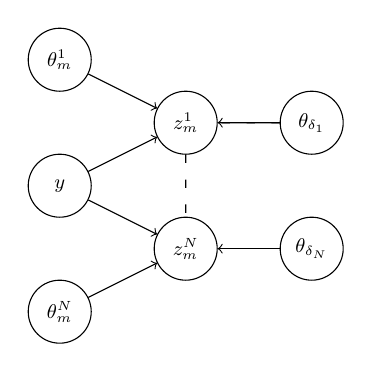
\begin{tikzpicture}[scale=0.8,every node/.style={transform shape}]
[inner sep=1mm] 
[line width=1pt]
\path (0,0) node (y) [shape=circle,minimum size=1cm,draw] {\small $y$};
\path (2,1) node (zm1) [shape=circle,minimum size=1cm,draw] {\small $z_m^1$};
\path (0,2) node (thetam1) [shape=circle,minimum size=1cm,draw] {\small $\theta_m^1$};
\path (2,-1) node (zmN) [shape=circle,minimum size=1cm,draw] {\small $z_m^N$};
\path (0,-2) node (thetamN) [shape=circle,minimum size=1cm,draw] {\small $\theta_m^N$};
\path (4,1) node (thetad1) [shape=circle,minimum size=1cm,draw] {\small $\theta_{\delta_1}$};
\path (4,-1) node (thetadN) [shape=circle,minimum size=1cm,draw] {\small $\theta_{\delta_N}$};


\draw [->] (thetam1) to (zm1);
\draw [->] (y) to (zm1);
\draw [->] (y) to (zmN);
\draw [->] (thetamN) to (zmN);
\draw [->] (thetad1) to (zm1);
\draw [->] (thetadN) to (zmN);

\draw [loosely dashed] (zm1) to (zmN);
\draw [loosely dashed] (thetad1) to (zm1);
\draw [loosely dashed] (thetadN) to (zmN);
\end{tikzpicture}
\end{figure}

\noindent This framework is related to the Reliability Ensemble Average approach where each model is weighted according to its reliability (given through the variance of $\epsilon_i$) which may be estimated empirically \citep{Giorgi_2002}. Note that a present-day observation model can be easily included in this model setup \citep[see also][]{Smith_2009,Tebaldi_2007}. A more elaborate version of the example given here including space-time dynamics is given in \cite{Berliner_2008}.

\demo


\end{document}



